% Copyright 2026 Sreeram Anil
% SPDX-License-Identifier: CC-BY-4.0
\chapter{Dual extended Kalman filter (Dual EKF)}
\label{ch:dualekf}

\section*{At a glance}
\begin{tabular}{@{}l>{\raggedright\arraybackslash}p{0.76\textwidth}@{}}
Family & Joint/dual state--parameter estimation (SOH) \\
Header & \texttt{include/estkit/parameter/dual\_ekf.hpp} \\
Registered name & \texttt{DualEKF} \\
State dimension & two filters: $n_x=4$ (state) and $n_p=2$ (parameters) \\
Cost per step & $\mathcal{O}(n_x^3+n_p^3+n_x^2 n_p)$; \SI{1.12}{\micro\second}/step measured, no heap \\
Primary references & \cite{plett2004ekf3,wannelson2001dual,ljung1979ekf} \\
\end{tabular}

\section{Motivation and aerospace/BMS relevance}
The joint filter of Chapter~\ref{ch:jointekf} puts the state and the parameters into one covariance
matrix.  That is elegant but it has two practical consequences.  First, the cost is cubic in
$n_x+n_p$: for a pack model with a dozen parameters the augmented filter becomes expensive, whereas
two smaller filters cost $n_x^3+n_p^3$.  Second, and more important in practice, the single
covariance forces a single tuning: the process-noise and measurement-noise assumptions that make
the state estimate well behaved are not the ones that make the parameter estimate well behaved, and
in the joint filter there is no way to separate them.

The \emph{dual} formulation, introduced for neural-network training by Wan and
Nelson~\cite{wannelson2001dual} and for battery management by Plett~\cite{plett2004ekf3}, runs two
coupled EKFs: one over $\vx$ with $\vtheta$ held at its current estimate, and one over $\vtheta$
whose ``measurement'' is the \emph{state filter's own output prediction}.  Each has its own
covariance, its own process noise and its own measurement noise, so the parameter filter can be made
deliberately slow and conservative --- which is what a BMS wants, because capacity changes over
months while SOC changes over seconds.

The subtlety, and the whole content of the method, is that the parameter filter's output Jacobian is
not $\partial h/\partial\vtheta$.  Changing $\vtheta$ changes the state estimate too, because the
state filter has been running with that $\vtheta$ since the beginning of the record.  The correct
sensitivity is a \emph{total} derivative, and computing it recursively is Plett's contribution.

\section{Problem statement and assumptions}
The plant is again \eqref{eq:je-f}--\eqref{eq:je-h} with the random walk of
Assumption~\ref{as:je-rw}.  We now maintain two estimates:
\begin{itemize}[nosep]
\item the state filter $(\xhat_k,\mP_k)$, an ordinary EKF on
      $\vx_{k+1}=f(\vx_k,\vu_k;\hat{\vtheta})$, $\vy_k=h(\vx_k,\vu_k;\hat{\vtheta})$;
\item the parameter filter $(\hat{\vtheta}_k,\bm{\Sigma}_{\theta,k})$, an EKF on
      $\vtheta_{k+1}=\vtheta_k+\bm{r}_k$ whose measurement model is
      $\vy_k=\hat{\vy}_k(\vtheta)+\bm{e}_k$ with
      $\hat{\vy}_k(\vtheta)=h(\xminus_k(\vtheta),\vu_k;\vtheta)$.
\end{itemize}

\begin{assumption}[Frozen gain]\label{as:de-gain}
The dependence of the state filter's Kalman gain $\mK_k$ on $\vtheta$ is neglected in the
sensitivity recursion, i.e.\ $\partial\mK_k/\partial\vtheta\approx\bm{0}$.  This is the
approximation made in both \cite{plett2004ekf3} and \cite{wannelson2001dual}; it is exact for a
steady-state gain and is an excellent approximation whenever the parameter estimate moves slowly
compared with the filter's convergence.
\end{assumption}

\begin{assumption}[Parameter-filter measurement noise]\label{as:de-R}
The residual $\vy_k-h(\xminus_k,\vu_k;\hat{\vtheta})$ seen by the parameter filter contains the
state estimation error as well as the sensor noise; its covariance is therefore taken as the state
filter's innovation covariance $\mR_\theta=\mH\mP^-_k\mH^\T+\mR$ rather than $\mR$ alone.
\end{assumption}

\section{Derivation}

\subsection{The two cost functions}
The dual formulation can be read as alternating minimisation of two coupled least-squares problems
\cite{wannelson2001dual}:
\begin{equation}
\min_{\vx_{0:k}} \sum_{j\le k}\norm{\vy_j-h(\vx_j,\vu_j;\hat{\vtheta})}^2_{\mR\inv}+\dots
\qquad\text{and}\qquad
\min_{\vtheta} \sum_{j\le k}\norm{\vy_j-\hat{\vy}_j(\vtheta)}^2_{\mR_\theta\inv},
\label{eq:de-costs}
\end{equation}
the first solved recursively by the state EKF and the second by the parameter EKF.  The parameter
problem is a \emph{prediction-error} problem in exactly Ljung's sense~\cite{ljung1979ekf}: the
predictor $\hat{\vy}_j(\vtheta)$ is the output of a filter driven by the whole past, so its
gradient with respect to $\vtheta$ must be propagated recursively.

\subsection{The total-derivative recursion}
Define the sensitivity matrices
\begin{equation}
\bm{\Psi}^-_k=\frac{\partial\xminus_k}{\partial\vtheta}\in\real^{n_x\times n_p},\qquad
\bm{\Psi}^+_k=\frac{\partial\xplus_k}{\partial\vtheta}\in\real^{n_x\times n_p},\qquad
\mC_k=\frac{\partial\hat{\vy}_k}{\partial\vtheta}\in\real^{n_y\times n_p}.
\label{eq:de-psi}
\end{equation}
Differentiating the state filter's own recursions with respect to $\vtheta$ and using
Assumption~\ref{as:de-gain} gives Plett's three equations~\cite[Part 3, §4]{plett2004ekf3}:
\begin{align}
\bm{\Psi}^-_k &= \left.\frac{\partial f}{\partial\vtheta}\right|_{\xplus_{k-1},\vu_{k-1}}
                 +\left.\frac{\partial f}{\partial\vx}\right|_{\xplus_{k-1},\vu_{k-1}}\bm{\Psi}^+_{k-1},
\label{eq:de-r1}\\
\mC_k &= \left.\frac{\partial h}{\partial\vtheta}\right|_{\xminus_k,\vu_k}
        +\left.\frac{\partial h}{\partial\vx}\right|_{\xminus_k,\vu_k}\bm{\Psi}^-_k,
\label{eq:de-r2}\\
\bm{\Psi}^+_k &= \bm{\Psi}^-_k-\mK_k\,\mC_k .
\label{eq:de-r3}
\end{align}
Equation \eqref{eq:de-r1} says that a change in $\vtheta$ affects the predicted state both directly
(through the dynamics) and indirectly (because the previous estimate already depended on
$\vtheta$); \eqref{eq:de-r2} propagates that into the output; \eqref{eq:de-r3} is the key step ---
the measurement update \emph{removes} part of the sensitivity, because the filter has already used
the measurement to correct whatever the parameter change did to the state.

\begin{remark}[Why \eqref{eq:de-r3} matters]\label{rem:de-r3}
For the ECM, $R_0$ does not appear in $f$, so $\partial f/\partial R_0=\bm{0}$ and, without
\eqref{eq:de-r3}, $\mC$ would simply be
$\partial h/\partial R_0=-\mathrm{arr}(T)\,i$, which at $i=\SI{22}{\ampere}$ is huge.  With
\eqref{eq:de-r3} the first measurement update sets
$\bm{\Psi}^+_{\soc,R_0}=-K_\soc\,\partial h/\partial R_0>0$ and at the next step
$\mC=\partial h/\partial R_0+(\partial h/\partial\soc)\bm{\Psi}^-_{\soc,R_0}\approx0$: the state
filter has already compensated a hypothetical $R_0$ change by moving the SOC, so the \emph{net}
effect of $R_0$ on the prediction is small and the parameter filter correctly refuses to make a
large correction.  Chapter~\ref{ch:dualukf} shows what happens when this cancellation is omitted.
\end{remark}

\subsection{The parameter filter}
With $\mC_k$ in hand the parameter filter is an ordinary EKF of dimension $n_p$:
\begin{align}
\bm{\Sigma}^-_{\theta,k}&=\bm{\Sigma}^+_{\theta,k-1}+\bm{\Sigma}_r, \label{eq:de-tu}\\
\mS_{\theta,k}&=\mC_k\bm{\Sigma}^-_{\theta,k}\mC_k^\T+\mR_\theta,\qquad
\mL_{\theta,k}=\bm{\Sigma}^-_{\theta,k}\mC_k^\T\mS_{\theta,k}\inv, \label{eq:de-gain}\\
\hat{\vtheta}^+_k&=\hat{\vtheta}^-_k+\mL_{\theta,k}\left(\vy_k-h(\xminus_k,\vu_k;\hat{\vtheta}^-_k)\right), \label{eq:de-upd}\\
\bm{\Sigma}^+_{\theta,k}&=(\mI-\mL_{\theta,k}\mC_k)\bm{\Sigma}^-_{\theta,k}(\mI-\mL_{\theta,k}\mC_k)^\T+\mL_{\theta,k}\mR_\theta\mL_{\theta,k}^\T . \label{eq:de-cov}
\end{align}

\subsection{Covariance matching: an adaptive parameter-filter noise for model error}
\label{sec:de-adapt}
Assumption~\ref{as:de-R} is still optimistic in one important respect.  It accounts for the
\emph{state} estimation error inside the residual, but it still assumes that whatever is left is the
white sensor noise $\mR$.  On a real cell it is not: an equivalent circuit is a two-time-constant
approximation of a distributed electrochemical system, and the part of the residual it cannot
represent is a \emph{structured, current-correlated} signal of a few millivolts.  That signal is
precisely the input the total derivative \eqref{eq:de-r2} is most sensitive to, so a parameter filter
that believes $\mR_\theta\approx\mR$ will integrate model error into $\hat{\vtheta}$ at full gain.

The standard remedy is covariance matching: choose the measurement-noise covariance so that the
\emph{observed} innovation statistics agree with the ones the filter predicts (Mehra~\cite{mehra1970};
Mohamed \& Schwartz~\cite{mohamed1999adaptive}).  Maintain an exponentially weighted estimate of the
actual squared residual,
\begin{equation}
\hat{\mR}_{\nu,k}=\rho\,\hat{\mR}_{\nu,k-1}+(1-\rho)\,\bm{e}_k\bm{e}_k^\T,
\qquad \bm{e}_k=\vy_k-h(\xminus_k,\vu_k;\hat{\vtheta}^-_k),
\label{eq:de-rhat}
\end{equation}
and \emph{floor} the parameter filter's measurement-noise covariance with it:
\begin{equation}
\boxed{\;\left[\mR_\theta\right]_{jj}=\max\left(\left[\mH\mP^-_k\mH^\T+\mR\right]_{jj},\;\left[\hat{\mR}_{\nu,k-1}\right]_{jj}\right)\;}
\label{eq:de-radapt}
\end{equation}
The statistic is updated \emph{after} it has been used at step $k$, so a genuine parameter error is
not allowed to inflate its own noise floor instantly.

Equation~\eqref{eq:de-radapt} is self-discriminating, which is why it is preferable to a fixed
inflation factor or to a hard innovation gate.  When the parameters are genuinely wrong ---
\texttt{aged\_cell}, where the commissioned resistance is \SI{27}{\percent} low --- the residual
starts at about \SI{4}{\milli\volt}, $\mR_\theta$ is inflated about threefold, and the filter
converges more slowly; but $\bm{\Sigma}_\theta$ is still large, so
$\mC\bm{\Sigma}_\theta\mC^\T$ dominates $\mS_\theta$ and the gain remains close to the
``explain it with $\vtheta$'' solution.  As the parameters are corrected the residual falls to about
\SI{1}{\milli\volt}, the floor deactivates and the filter sharpens again.  When the residual is
structural model error, $\bm{\Sigma}_\theta$ collapses but the residual does \emph{not}, so the floor
stays active permanently and the parameter filter stays slow.  In other words, the mechanism asks
``did the last hundred seconds of parameter updates actually reduce the residual?'' and throttles
itself when the answer is no.

A second, cheaper safeguard bounds $\bm{\Sigma}_\theta$ from above by the commissioning prior,
\begin{equation}
\left[\bm{\Sigma}^+_\theta\right]_{kk}\le\left[\bm{\Sigma}_\theta(0)\right]_{kk} ,
\label{eq:de-ceiling}
\end{equation}
implemented as a symmetric rescaling of row and column $k$ so that the matrix stays a valid
covariance.  The prior is a physical statement (``the capacity is within \SI{10}{\percent} of
nameplate''), and a filter that has become \emph{less} certain than that, through repeated random-walk
additions in an unexciting segment, has lost more than it has learned.  On this benchmark the ceiling
never activates --- the results are bit-identical with it disabled --- but it costs one comparison per
step and removes an unbounded failure mode on missions with long low-current phases.

\subsection{Sequencing}
Plett's ordering~\cite[Part 3, Table 4]{plett2004ekf3} is followed exactly:
parameter time update \eqref{eq:de-tu} $\rightarrow$ sensitivity propagation \eqref{eq:de-r1}
$\rightarrow$ state time update $\rightarrow$ parameter measurement update
\eqref{eq:de-r2}--\eqref{eq:de-cov} $\rightarrow$ state measurement update $\rightarrow$
sensitivity posterior \eqref{eq:de-r3}.  The updated $\hat{\vtheta}^+_k$ is written into the state
filter's model only \emph{after} the state update, so the whole of step $k$ is executed with a
single, consistent parameter vector.

\subsection{Parameter derivatives}
$\partial f/\partial\vtheta$ and $\partial h/\partial\vtheta$ are central differences taken through
\texttt{set\_params()}, \eqref{eq:je-fd}, with a relative step $\varepsilon=10^{-4}$.  The larger
step (compared with the joint EKF's $10^{-6}$) is deliberate: $f$ is almost exactly affine in $1/Q$
and $h$ exactly affine in $R_0$, so the truncation error is negligible while the cancellation error
--- which for $\partial f_\soc/\partial Q\approx6\times10^{-6}$ is the binding constraint --- is
reduced by two orders of magnitude.  This also keeps the single-precision build meaningful.

\section{Algorithm}
\begin{algorithm}[H]
\caption{Dual EKF --- one sampling period}
\begin{algorithmic}[1]
\Require $\xplus_{k-1},\mP^+_{k-1},\hat{\vtheta}^+_{k-1},\bm{\Sigma}^+_{\theta,k-1},\bm{\Psi}^+_{k-1},\vu_{k-1},\vy_k,\vu_k$
\State \textbf{Parameter time update:} $\hat{\vtheta}^-_k\gets\hat{\vtheta}^+_{k-1}$, $\bm{\Sigma}^-_\theta\gets\bm{\Sigma}^+_\theta+\bm{\Sigma}_r$
\State \textbf{Sensitivity:} $\bm{\Psi}^-_k\gets\partial f/\partial\vtheta+(\partial f/\partial\vx)\,\bm{\Psi}^+_{k-1}$ \Comment{Eq.\ \eqref{eq:de-r1}}
\State \textbf{State time update:} $\xminus_k\gets f(\xplus_{k-1},\vu_{k-1};\hat{\vtheta}^-_k)$, $\mP^-_k\gets\mF\mP^+_{k-1}\mF^\T+\mQ$
\State \textbf{Parameter measurement update:} $\mC_k\gets\partial h/\partial\vtheta+(\partial h/\partial\vx)\bm{\Psi}^-_k$
\State $\mR_\theta\gets\max\!\left(\mH\mP^-_k\mH^\T+\mR,\ \hat{\mR}_\nu\right)$ elementwise on the diagonal \Comment{Eq.\ \eqref{eq:de-radapt}}
\State $\mS_\theta,\mL_\theta\gets$ \eqref{eq:de-gain}
\State $\hat{\vtheta}^+_k\gets\hat{\vtheta}^-_k+\mL_\theta(\vy_k-h(\xminus_k,\vu_k;\hat{\vtheta}^-_k))$, clamp to the box; $\bm{\Sigma}^+_\theta\gets$ \eqref{eq:de-cov}
\State \textbf{State measurement update:} standard EKF with Joseph covariance, gain $\mK_k$
\State cap $\bm{\Sigma}^+_\theta$ at the prior \eqref{eq:de-ceiling}; update $\hat{\mR}_\nu$ by \eqref{eq:de-rhat}
\State $\bm{\Psi}^+_k\gets\bm{\Psi}^-_k-\mK_k\mC_k$; write $\hat{\vtheta}^+_k$ into the state filter's model
\Ensure $\xplus_k,\mP^+_k,\hat{\vtheta}^+_k,\bm{\Sigma}^+_{\theta,k},\bm{\Psi}^+_k$
\end{algorithmic}
\end{algorithm}

\section{Application to the battery model}
The state filter is \texttt{Ekf<EcmModel>} and the parameter filter is a $2\times2$ recursion over
$\vtheta=[Q,R_0]^\T$.  The priors and the random walk are identical to the joint filters
(Section~\ref{sec:je-app}) so that the three methods can be compared directly:
$p_{0,Q}=(0.10\,Q_\text{nom})^2$, $q_Q=(\SI{5e-5}{\ampere\hour})^2$ per step,
$p_{0,R_0}=(0.30\,R_{0,\text{nom}})^2$, $q_{R_0}=(\SI{2e-6}{\ohm})^2$ per step, boxes
$Q\in[0.5,1.5]\,Q_\text{nom}$ and $R_0\in[0.2,5]\,R_{0,\text{nom}}$.

$\mR_\theta$ deserves a comment.  Taking $\mR_\theta=\mR$ (the sensor noise alone) makes the
parameter filter grossly over-confident during the first seconds, when the residual is dominated by
the unknown hysteresis state and the RC voltages rather than by the parameters; in that regime
$\mL_\theta\approx\mC^{-1}$ and a \SI{20}{\milli\volt} transient is converted into a
\SI{20}{\milli\ohm} correction, which saturates $R_0$ against its box.  Using Assumption
\ref{as:de-R}, $\mR_\theta=\mH\mP^-\mH^\T+\mR$, the same transient is correctly attributed to the
state, because at $k=0$ the SOC variance is $\sigma_{\soc,0}^2=0.01$ and
$\mH\mP^-\mH^\T\approx\SI{4.9e-3}{\volt\squared}$ dominates $\mR\approx\SI{4.4e-6}{\volt\squared}$
by three orders of magnitude.  The option is exposed as \texttt{innovation\_covariance} and is on by
default.  A further fixed inflation factor \texttt{r\_theta\_scale} is available but is left at $1$,
because the adaptive floor of Section~\ref{sec:de-adapt} supersedes it.

The adaptive floor \eqref{eq:de-radapt} is enabled by default (\texttt{adapt\_r\_theta}) with a
forgetting factor $\rho=0.999$, i.e.\ an effective memory of $1000$ samples or \SI{100}{\second} at
the benchmark's \SI{10}{\hertz} rate.  The choice is not arbitrary and the method is genuinely
sensitive to it, because $\rho$ sets the time scale on which ``the residual is still large'' is
judged.  Measured over three seeds on both plants:
\begin{center}
\begin{tabular}{@{}lccccc@{}}
\toprule
 & $\rho=0.99$ & $\rho=0.995$ & $\rho=0.999$ & $\rho=0.9998$ & (floor off)\\
\midrule
ECM \texttt{nominal} $\text{RMSE}_\text{ss}$      & $0.0020$ & $0.0004$ & $0.0008$ & $0.0008$ & $0.0016$\\
ECM \texttt{aged\_cell} $\text{RMSE}_\text{ss}$   & $0.0045$ & $0.0034$ & $0.0066$ & $0.0186$ & $0.0025$\\
SPM \texttt{nominal} $\text{RMSE}_\text{ss}$      & $0.1024$ & $0.0977$ & $\mathbf{0.0086}$ & $0.0247$ & $0.1167$\\
SPM \texttt{cold} $\text{RMSE}_\text{ss}$         & $0.0717$ & $0.0477$ & $\mathbf{0.0206}$ & $0.0429$ & $0.1364$\\
\bottomrule
\end{tabular}
\end{center}
A memory shorter than about a minute lets the statistic relax between the mission's high-current
transients, so the filter becomes over-confident again just before the next one and the SPM failure
returns; a memory much longer than the mission averages away the very drop in residual that signals
successful convergence, and \texttt{aged\_cell} degrades.  \SI{100}{\second} sits between the
duration of the mission's fastest segments (\SIrange{45}{75}{\second}) and that of the mission itself,
and is the knee of both curves.

An innovation gate on the parameter update (\texttt{innov\_gate}) is also implemented but disabled.
On this mission the voltage residual during the high-current transients is dominated by ECM model
error, not by sensor noise, so any gate tight enough to reject a \SI{50}{\milli\volt} outlier also
rejects the most informative samples; with a $5\sigma$ gate the nominal steady-state SOC RMSE rose
from $0.0011$ to $0.0131$.  A gate is a hard, threshold-dependent decision taken on a single sample;
the adaptive floor \eqref{eq:de-radapt} achieves the same end continuously and without a threshold,
which is why it is the mechanism that is enabled.

\section{Implementation notes}
Storage is \SI{4752}{\byte}: one \texttt{Ekf<EcmModel>} plus $\bm{\Sigma}_\theta,\bm{\Sigma}_r$ and
the prior variances ($2\times2$ each), $\bm{\Psi}^\pm$ ($4\times2$ each) and the $1\times1$ residual
statistic $\hat{\mR}_\nu$.  The measured cost is \SI{1.27}{\micro\second}/step, the cheapest of the
four joint/dual filters and $2.6\times$ the plain EKF; the $2\times2$ parameter algebra is negligible
and the cost is dominated by the $2n_p$ model copies in the central differences.  The adaptive floor
adds one multiply--add and one comparison per step.  The Joseph form is used for both covariances,
both are symmetrised, and every update is guarded: if $\mS_\theta$ is singular or the update is not
finite the parameter step is skipped and the state filter proceeds, so a numerical failure degrades
the method to a plain EKF rather than to divergence.

The remaining structural limitation is Assumption~\ref{as:de-gain}: the sensitivity recursion
discards $\partial\mK/\partial\vtheta$, so when the parameters move fast it lags the truth and
$\mL_\theta$ is mis-scaled.  The second limitation of the original formulation --- that the parameter
filter consumes a residual which is only white if the model is correct --- is what
Section~\ref{sec:de-adapt} addresses; it is mitigated, not removed.  The filter still cannot
\emph{separate} model error from parameter error, it can only detect that the two together are
larger than the sensor model admits and slow down accordingly.  On a plant whose model error happens
to be perfectly correlated with a parameter direction, the estimate would still be biased --- slowly.

\section{Benchmark results}
\label{sec:de-results}
% Copyright 2026 Sreeram Anil
% SPDX-License-Identifier: CC-BY-4.0
\begin{table}[H]\centering\footnotesize\setlength{\tabcolsep}{4pt}
\caption{DualEKF: cell-level benchmark on the eVTOL mission (mean over seeds; RMSE and max error in \% SOC; $t_\mathrm{conv}$: first time the error stays below 2\,\% for 60\,s, -- = never; EKF reference: steady-state RMSE of the plain EKF on the same data).}\label{tab:cell_DualEKF}
\begin{tabular}{llrrrrrcrr}\toprule
plant & scenario & RMSE & RMSE$_\mathrm{ss}$ & max & $t_\mathrm{conv}$ [s] & RMSE$_v$ [mV] & div. & EKF ref. & ns/step \\ \midrule
ECM & nominal & 0.17 & 0.08 & 1.07 & 0 & 0.79 & no & 0.05 & 1272 \\
ECM & init\_error & 0.16 & 0.08 & 0.61 & 0 & 2.12 & no & 0.05 & 1272 \\
ECM & current\_bias & 0.66 & 0.79 & 1.42 & 0 & 0.80 & no & 0.61 & 1272 \\
ECM & noise\_step & 0.30 & 0.31 & 1.07 & 0 & 2.89 & no & 0.12 & 1277 \\
ECM & outliers & 0.43 & 0.34 & 3.04 & 3 & 2.06 & no & 0.21 & 1273 \\
ECM & cold & 0.34 & 0.41 & 1.17 & 0 & 1.90 & no & 0.16 & 1271 \\
ECM & hot & 0.19 & 0.07 & 1.03 & 0 & 0.55 & no & 0.03 & 1273 \\
ECM & aged\_cell & 0.69 & 0.66 & 1.37 & 0 & 1.16 & no & 1.52 & 1272 \\
ECM & param\_mismatch & 1.53 & 1.94 & 2.28 & 0 & 1.05 & no & 1.36 & 1273 \\
ECM & sensor\_dropout & 0.47 & 0.28 & 1.84 & 0 & 1.84 & no & 0.46 & 1273 \\
ECM & preisach & 0.91 & 0.94 & 2.04 & 29 & 0.80 & no & 0.20 & 1284 \\
ECM & combined & 3.67 & 2.01 & 10.26 & 414 & 2.30 & no & 12.44 & 1274 \\
\midrule
SPM & nominal & 1.78 & 0.86 & 3.47 & 0 & 0.85 & no & 3.73 & 1158 \\
SPM & init\_error & 2.00 & 0.86 & 4.01 & 0 & 2.09 & no & 3.81 & 1164 \\
SPM & current\_bias & 2.42 & 1.45 & 4.21 & 0 & 0.86 & no & 5.69 & 1171 \\
SPM & noise\_step & 1.95 & 1.52 & 3.71 & 0 & 3.09 & no & 3.30 & 1171 \\
SPM & outliers & 1.35 & 1.07 & 3.28 & 554 & 2.20 & no & 1.99 & 1171 \\
SPM & cold & 3.63 & 2.06 & 6.27 & 16 & 2.50 & no & 7.35 & 1172 \\
SPM & hot & 1.16 & 0.60 & 2.20 & 0 & 0.54 & no & 2.16 & 1166 \\
SPM & param\_mismatch & 1.99 & 1.18 & 3.59 & 0 & 0.88 & no & 3.13 & 1167 \\
SPM & sensor\_dropout & 3.07 & 1.69 & 5.47 & 0 & 1.98 & no & 5.31 & 1166 \\
\bottomrule\end{tabular}\end{table}
\begin{table}[H]\centering\small\caption{DualEKF: additional outputs (capacity error at the end of the mission in Ah, averaged over the last 10\,\% of the run; interval-bound violation rate).}\label{tab:cellx_DualEKF}
\begin{tabular}{llrr}\toprule plant & scenario & $\hat Q - Q$ [Ah] & bound violation [\%] \\ \midrule
ECM & nominal & +0.049 & -- \\
ECM & init\_error & +0.044 & -- \\
ECM & current\_bias & +0.415 & -- \\
ECM & noise\_step & +0.035 & -- \\
ECM & outliers & +0.005 & -- \\
ECM & cold & +0.026 & -- \\
ECM & hot & +0.057 & -- \\
ECM & aged\_cell & +0.054 & -- \\
ECM & param\_mismatch & +0.100 & -- \\
ECM & sensor\_dropout & +0.043 & -- \\
ECM & preisach & +0.244 & -- \\
ECM & combined & +0.104 & -- \\
SPM & nominal & +0.359 & -- \\
SPM & init\_error & +0.384 & -- \\
SPM & current\_bias & +0.835 & -- \\
SPM & noise\_step & +0.590 & -- \\
SPM & outliers & +0.144 & -- \\
SPM & cold & +1.093 & -- \\
SPM & hot & +0.303 & -- \\
SPM & param\_mismatch & +0.460 & -- \\
SPM & sensor\_dropout & +0.669 & -- \\
\bottomrule\end{tabular}\end{table}

\begin{figure}[H]\centering
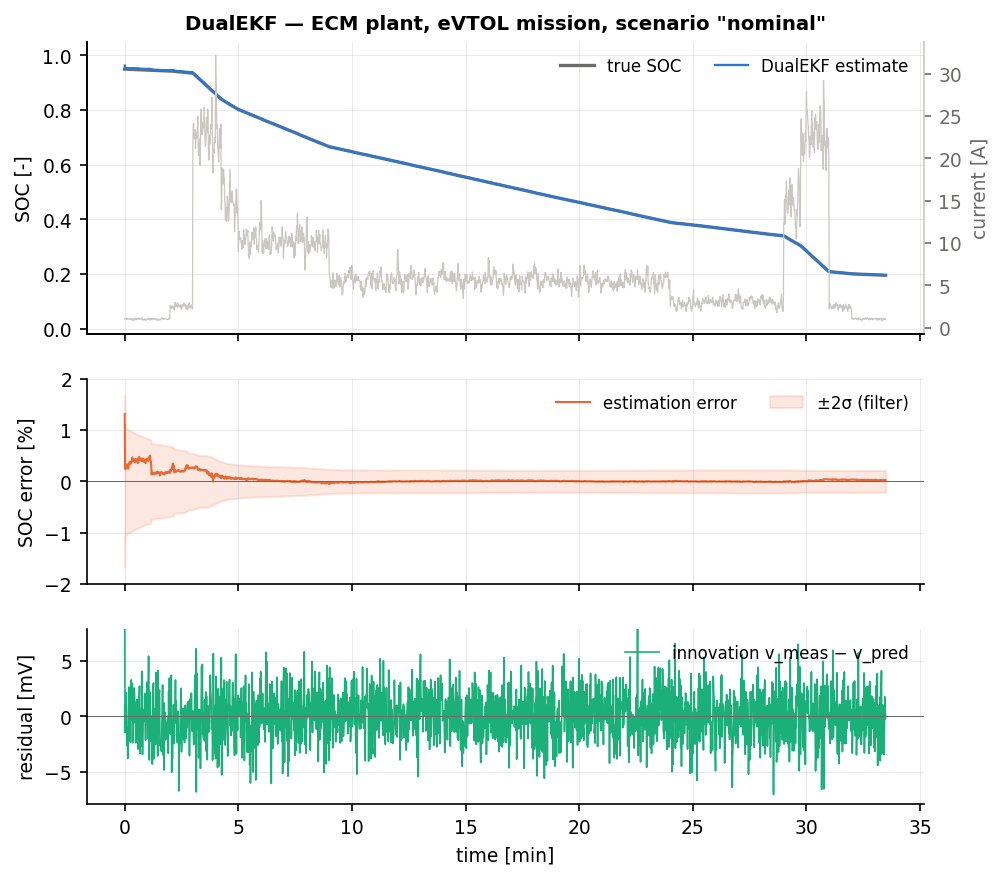
\includegraphics[width=\textwidth]{figures/cell_DualEKF_nominal.png}
\caption{DualEKF on the nominal eVTOL mission: true and estimated SOC (top), estimation error with the $\pm 2\sigma$ band (middle), voltage residual (bottom).}
\end{figure}
\begin{figure}[H]\centering
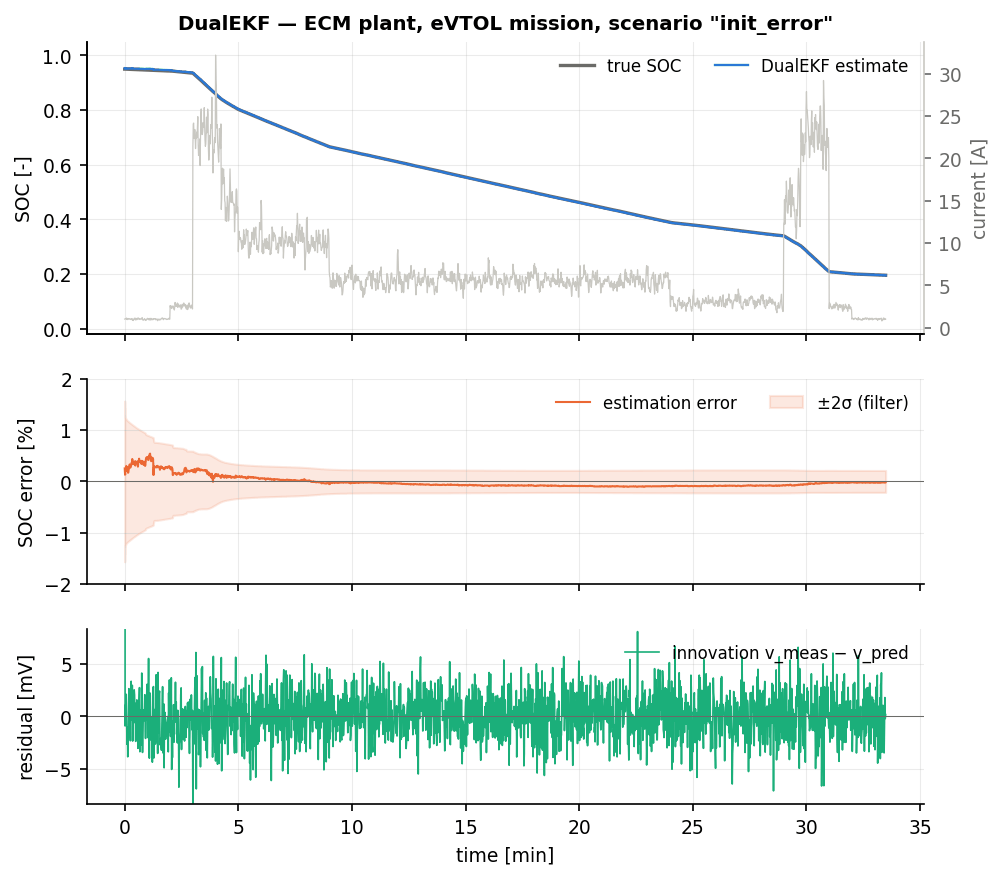
\includegraphics[width=\textwidth]{figures/cell_DualEKF_init_error.png}
\caption{DualEKF with a \SI{35}{\percent} initial SOC error.}
\end{figure}

All figures below are means over three seeds on the eVTOL profile.

\paragraph{ECM plant.}  On \texttt{nominal} the dual EKF reaches $\text{RMSE}=0.0017$ and
$\text{RMSE}_\text{ss}=0.0008$ with immediate convergence (plain EKF $0.0015/0.0005$, plain UKF
$0.0020/0.0004$).  On \texttt{init\_error} it converges at $t=0$ with $\text{RMSE}=0.0016$ ---
the best of the four joint/dual filters, and better than the plain EKF.  Both acceptance criteria are
met and no scenario diverges in any seed.

On \texttt{aged\_cell} it recovers most of the joint filters' advantage:
$\text{RMSE}_\text{ss}=0.0066$ against the plain EKF's $0.0152$, with
$\texttt{capacity\_err\_end}=\SI{+0.054}{\ampere\hour}$.  The three reference capacity figures are
\begin{center}
\begin{tabular}{@{}lrr@{}}
\toprule
Scenario & $Q_\text{true}$ (\si{\ampere\hour}) & \texttt{capacity\_err\_end} (\si{\ampere\hour})\\
\midrule
\texttt{nominal}      & 5.00 & $+0.049$\\
\texttt{aged\_cell}   & 4.25 & $+0.054$\\
\texttt{current\_bias}& 5.00 & $+0.415$\\
\bottomrule
\end{tabular}
\end{center}
As for every method in this family, the \texttt{current\_bias} figure measures the
unidentifiability of the product (sensor gain)$\times$(capacity)~\cite{zhao2017observability,lin2018sensorbias}
rather than an estimator defect.

The adaptive floor of Section~\ref{sec:de-adapt} changes the ECM picture in a way that is worth
reading carefully, because it is a textbook bias/variance trade:
\begin{center}
\begin{tabular}{@{}lccc@{}}
\toprule
ECM scenario ($\text{RMSE}_\text{ss}$) & floor off & floor on & plain EKF\\
\midrule
\texttt{nominal}        & $0.0016$ & $0.0008$ & $0.0005$\\
\texttt{aged\_cell}     & $0.0025$ & $0.0066$ & $0.0152$\\
\texttt{param\_mismatch}& $0.0332$ & $0.0194$ & $0.0136$\\
\texttt{sensor\_dropout}& $0.0213$ & $\mathbf{0.0028}$ & $0.0046$\\
\texttt{combined}       & $0.0284$ & $0.0201$ & $0.1244$\\
\bottomrule
\end{tabular}
\end{center}
The filter gives up a factor of about two on \texttt{aged\_cell} --- the one scenario in which the
residual really is pure parameter error, so throttling costs accuracy --- and buys back far more
everywhere the residual is not: a factor of $7.6$ on \texttt{sensor\_dropout}, where the
\SI{15}{\second} stuck voltage now raises $\hat{\mR}_\nu$ within a second and the parameter filter
simply stops listening (\texttt{capacity\_err\_end} improves from \SI{+0.261}{\ampere\hour} to
\SI{+0.043}{\ampere\hour}), and a factor of $1.7$ on \texttt{param\_mismatch}.  The
\texttt{aged\_cell} \emph{capacity} estimate, which is the quantity the method exists for, is
unaffected (\SI{+0.052}{\ampere\hour} before, \SI{+0.054}{\ampere\hour} after): the floor slows the
parameter filter down but does not stop it reaching the right answer when there is one.

\paragraph{Behaviour under model mismatch: the electrochemical plant.}
\label{sec:de-spm}
The decisive test is the single-particle-model plant, where the estimator runs an ECM fitted to an
electrochemical cell and therefore carries a structured voltage model error of a few millivolts that
\emph{no} value of $\vtheta$ can remove.  Without the adaptive floor the dual EKF was the worst
estimator in the whole benchmark on that plant: the parameter filter integrates the model error, the
capacity estimate is dragged from \SI{5.07}{\ampere\hour} to \SI{3.75}{\ampere\hour} during the
\SI{4.5}{C} take-off hover, and the SOC locks at $-10\,\%$ for the rest of the mission.  With the
floor enabled (means over three seeds, SPM plant):
\begin{center}
\begin{tabular}{@{}lrrrrr@{}}
\toprule
SPM scenario ($\text{RMSE}_\text{ss}$) & DualEKF, floor off & \textbf{DualEKF} & plain EKF & JointEKF & JointUKF\\
\midrule
\texttt{nominal}        & $0.1167$ & $\mathbf{0.0086}$ & $0.0373$ & $0.0211$ & $0.0140$\\
\texttt{init\_error}    & $0.0888$ & $\mathbf{0.0086}$ & $0.0381$ & $0.0166$ & $0.0082$\\
\texttt{current\_bias}  & $0.1343$ & $\mathbf{0.0145}$ & $0.0569$ & $0.0314$ & $0.0151$\\
\texttt{cold}           & $0.1364$ & $\mathbf{0.0206}$ & $0.0735$ & $0.0319$ & $0.0249$\\
\texttt{param\_mismatch}& $0.1220$ & $\mathbf{0.0118}$ & $0.0313$ & $0.0237$ & $0.0092$\\
\texttt{sensor\_dropout}& $0.0936$ & $\mathbf{0.0169}$ & $0.0531$ & $0.0225$ & $0.0220$\\
\bottomrule
\end{tabular}
\end{center}
The dual EKF goes from the worst estimator on that plant to the best: \emph{a factor of
thirteen} on \texttt{nominal}, and four times better than the plain EKF it wraps.  Its worst
steady-state error over the nine SPM scenarios and three seeds is $0.0230$, against $0.0804$ for the
plain EKF.  The reason it ends up ahead of the plain EKF rather than merely level with it is that the
throttled parameter filter still has enough authority to absorb the \emph{slowly varying} part of the
mismatch (an effective $R_0$ and an effective capacity for the fitted ECM) while refusing the fast,
current-correlated part --- which is exactly the separation the covariance-matching criterion is
designed to make.

\paragraph{Multi-flight capacity tracking.}  Over a 120-flight accelerated ageing study
(\texttt{bench\_soh --flights 120 --accel 3}), in which the true capacity falls from \SI{5.00}{} to
\SI{3.95}{\ampere\hour}, the dual EKF tracks it with a capacity RMSE of \SI{25.5}{\milli\ampere\hour}
over flights $11$--$120$ and a final error of \SI{+29}{\milli\ampere\hour} --- the best of the four
joint/dual filters (JointEKF \SI{26.3}{}, JointUKF \SI{28.7}{}, DualUKF \SI{33.0}{\milli\ampere\hour}),
at the same cost as the joint EKF (\SI{1.76}{} against \SI{1.75}{\micro\second} per step in
this benchmark) and with the smallest state of the four.  The residual \SI{+29}{\milli\ampere\hour} is the irreducible
\SI{+0.5}{\percent} current-sensor scale-factor bias.  Its mean per-flight SOC RMSE over the study is
$0.0042$.

Cost: \SI{1.27}{\micro\second}/step and \SI{4752}{\byte} --- the cheapest SOH method in this family
that also estimates capacity.

\section{Summary}
The dual EKF is the pragmatic choice for a flight BMS.  On the equivalent-circuit plant it delivers
most of the joint filter's improvement on an aged cell and a capacity estimate good to
\SI{0.05}{\ampere\hour} for $2.6\times$ the cost of a plain EKF, it is the best of the four
joint/dual filters at recovering from a large initial state error, and over a 120-flight ageing study
it tracks a fading capacity to \SI{25}{\milli\ampere\hour}, the best of the family.  Its decisive
property, though, is what happens when the cell model is simply wrong: with the innovation-based
covariance-matching floor of Section~\ref{sec:de-adapt} it is the \emph{best} estimator in the whole
benchmark on the electrochemical plant ($\text{RMSE}_\text{ss}=0.0086$ against the plain EKF's
$0.0373$), where without it, it was the worst ($0.1167$).

Use it when the parameter count grows (its cost is $n_x^3+n_p^3$, not $(n_x+n_p)^3$), when the
parameter tracking rate must be tuned independently of the state filter, or --- above all --- when
the cell model is an approximation whose residual is not white, which is every real cell.  Do not
disable the adaptive floor, and do not replace it with a fixed inflation factor or an innovation
gate: both were measured and both are worse, because the right amount of throttling is not known in
advance and changes during the mission.  Remember that the floor mitigates rather than removes the
underlying difficulty: the filter can tell that model and parameter error together exceed the sensor
model, but it cannot tell the two apart, so a model error aligned with a parameter direction will
still bias $\hat{\vtheta}$ --- slowly.  And, as with every method in this family, the capacity it
reports is the product of the true capacity and the current-sensor scale factor.
